\documentclass[12pt]{Qual}
\usepackage{preamble}

\name{Kayla Orlinsky}
\course{Complex Analysis Exam}
\term{Spring 2016}
\hwnum{Spring 2016}

\begin{document}

\begin{problem} $\,$
Let $a\in\mathbb{C}$ be such that $0<|a|<1,$ and set $$f(z)=\frac{1-z^2}{z^2-(a+\frac{1}{a})z+1}.$$ Find the Laurent expansion of $f$ in a neighborhood of the unit circle $|z|=1.$
\end{problem}


\begin{solution}$\,$
We interpret ``A neighborhood of the unit circle'' to actually mean for some $B_r(0)\subset\mathbb{D}$.

First, \begin{align*}
    z^2-(a+\frac{1}{a})z+1&=0\\
    \implies z&=\frac{a+\frac{1}{a}\pm\sqrt{(a+\frac{1}{a})^2-4}}{2}\\
    &=\frac{a+\frac{1}{a}\pm\sqrt{a^2+2+\frac{1}{a^2}-4}}{2}\\
    &=\frac{a+\frac{1}{a}\pm\sqrt{a^2-2+\frac{1}{a^2}}}{2}\\
    &=\frac{a+\frac{1}{a}\pm\sqrt{(a-\frac{1}{a})^2}}{2}\\
    &=\frac{a+\frac{1}{a}\pm(a-\frac{1}{a})}{2}\\
    &=a,\frac{1}{a}
\end{align*}

Thus, $$f(z)=\frac{(1-z^2)}{(z-a)(z-\frac{1}{a})}.$$

Now, \begin{align*}
    f(z)&=(1-z^2)\left[\frac{\frac{a}{a^2-1}}{z-a}-\frac{\frac{a}{a^2-1}}{z-\frac{1}{a}}\right]\\
    &=(1-z^2)\left[\frac{\frac{a}{a^2-1}}{-a(1-\frac{z}{a})}-\frac{\frac{a}{a^2-1}}{\frac{1}{a}(1-az)}\right]\\
    &=(1-z^2)\left[\frac{\frac{a^2}{a^2-1}}{1-az}-\frac{\frac{1}{a^2-1}}{1-\frac{z}{a}}\right]\\
\end{align*}

Now, for $|z|<|a|$, we have that $|az|<|a|^2<1$ and $\frac{|z|}{|a|}<1$.

Thus, on $\{|z|<|a|\}$, $$\frac{\frac{a^2}{a^2-1}}{1-az}=\frac{a^2}{a^2-1}\sum_{n=0}^\infty(az)^n$$ and $$\frac{\frac{1}{a^2-1}}{1-\frac{z}{a}}=\frac{1}{a^2-1}\sum_{n=0}^\infty\left(\frac{z}{a}\right)^n$$

so \begin{align*}
    f(z)&=(1-z^2)\sum_{n=0}^\infty\left[\frac{a^2}{a^2-1}a^n-\frac{a^{-n}}{a^2-1}\right]z^n\\
    &=(1-z^2)\sum_{n=0}^\infty\left[\frac{a^{n+2}-a^{-n}}{a^2-1}\right]z^n\\
    &=(1-z^2)\sum_{n=0}^\infty \alpha_nz^n\qquad\qquad\qquad \alpha_n=\frac{a^{n+2}-a^{-n}}{a^2-1}\\
    &=\sum_{n=0}^\infty \alpha_nz^n-\sum_{n=0}^\infty \alpha_nz^{n+2}\\
    &=\sum_{n=0}^\infty \alpha_nz^n-\sum_{k=-2}^\infty \alpha_{k+2}z^k\\
    &=\sum_{n=0}^\infty \alpha_nz^n-\alpha_0z^{-2}-\alpha_1z^{-1}-\sum_{k=0}^\infty \alpha_{k+2}z^k\\
    &=-\alpha_0z^{-2}-\alpha_1z^{-1}+\sum_{n=0}^\infty \alpha_nz^n-\sum_{n=0}^\infty \alpha_{n+2}z^n\\
    &=-\alpha_0z^{-2}-\alpha_1z^{-1}+\sum_{n=0}^\infty(\alpha_n-\alpha_{n+2})z^n\\
    &=-z^{-2}-\frac{a^2+1}{a}z^{-1}+\sum_{n=0}^\infty(\alpha_n-\alpha_{n+2})z^n
\end{align*}

Alternatively, note that we could have interpreted ``A neighborhood of the unit circle'' to actually mean that we must find the Laurent expansion in some annulus $\{s<|z|<t\}$ with $s<1<t$ so the unit circle is contained in the annulus.

In this case, we would use that for $|a|<|z|<\frac{1}{|a|}$, so $\frac{|a|}{|z|}<1$ and $|az|<1$.

Then we would simply rewrite $f(z)$ to be \begin{align*}
    f(z)&=(1-z^2)\left[\frac{\frac{a}{a^2-1}}{z-a}-\frac{\frac{a}{a^2-1}}{z-\frac{1}{a}}\right]\\
    &=(1-z^2)\left[\frac{\frac{a}{a^2-1}}{z(1-\frac{a}{z})}-\frac{\frac{a}{a^2-1}}{\frac{1}{a}(1-az)}\right]\\
    &=(1-z^2)\left[\frac{\frac{1}{z}\frac{a}{a^2-1}}{1-\frac{a}{z}}-\frac{\frac{a^2}{a^2-1}}{1-az}\right]
\end{align*}

and so on $\{|a|<|z|<\frac{1}{|a|}\}$, which is an annulus containing the unit circle since $|a|<1<\frac{1}{|a|}$, $$\frac{\frac{1}{z}\frac{a}{a^2-1}}{1-\frac{a}{z}}=\frac{a}{a^2-1}\sum_{n=0}^\infty\frac{a^n}{z^{n+1}}$$ and $$\frac{\frac{a^2}{a^2-1}}{1-az}=\frac{a^2}{a^2-1}\sum_{n=0}^\infty(az)^n$$

\begin{align*}
    f(z)&=(1-z^2)\left[\frac{a}{a^2-1}\sum_{n=0}^\infty\frac{a^n}{z^{n+1}}-\frac{a^2}{a^2-1}\sum_{n=0}^\infty(az)^n\right]\\
    &=\frac{a}{a^2-1}\left[\sum_{n=0}^\infty\frac{a^n}{z^{n+1}}-\sum_{n=0}^\infty\frac{a^n}{z^{n-1}}\right]-\frac{a^2}{a^2-1}\left[\sum_{n=0}^\infty a^nz^n-\sum_{n=0}^\infty a^nz^{n+2}\right]\\
    &=\frac{a}{a^2-1}\left[\sum_{n=0}^\infty\frac{a^n}{z^{n+1}}-z-a-\sum_{n=2}^\infty\frac{a^n}{z^{n-1}}\right]-\frac{a^2}{a^2-1}\left[1+az+\sum_{n=2}^\infty a^nz^n-\sum_{n=0}^\infty a^nz^{n+2}\right]\\
    &=\frac{a}{a^2-1}\left[\sum_{n=0}^\infty\frac{a^n}{z^{n+1}}-z-a-\sum_{k=0}^\infty\frac{a^{k+2}}{z^{k+1}}\right]-\frac{a^2}{a^2-1}\left[1+az+\sum_{k=0}^\infty a^{k+2}z^{k+2}-\sum_{n=0}^\infty a^nz^{n+2}\right]\\
    &=\frac{a}{a^2-1}\left[-z-a+\sum_{n=0}^\infty\frac{a^n-a^{n+2}}{z^{n+1}}\right]-\frac{a^2}{a^2-1}\left[1+az+\sum_{n=0}^\infty (a^{n+2}-a^n)z^{n+2}\right]\\
    &=-\frac{a}{a^2-1}z-\frac{a^2}{a^2-1}+\frac{a}{a^2-1}\sum_{n=0}^\infty\frac{a^n-a^{n+2}}{z^{n+1}}-\frac{a^2}{a^2-1}-\frac{a^3}{a^2-1}z-\frac{a^2}{a^2-1}\sum_{n=0}^\infty (a^{n+2}-a^n)z^{n+2}\\
    &=-\frac{2a^2}{a^2-1}-\frac{a+a^3}{a^2-1}z+\frac{a}{a^2-1}\sum_{n=0}^\infty\frac{a^n-a^{n+2}}{z^{n+1}}-\frac{a^2}{a^2-1}\sum_{n=0}^\infty (a^{n+2}-a^n)z^{n+2}\\
\end{align*}
\end{solution}
\newpage



\begin{problem} $\,$
Let $a\in\mathbb{C}$ be such that $0<|a|<1$ and let $n\in\mathbb{N}$. Show that $e^z(z-1)^n=a$ has exactly $n$ simple roots in the half-plane $\{z\in\mathbb{C}:\re(z)>0\}.$
\end{problem}

\begin{solution}$\,$
First, note that if $z$ is in the right-half plane and $e^z(z-1)^n=a$ then \begin{align*}
    |z-1|^n&<|e^z||z-1|^n\qquad |e^z|=e^{\re(z)}>e^0=1\\
    &=|a|<1\\
    \implies |z-1|&<1
\end{align*} so if $f(z)=e^z(z-1)^n-a$ has a zero in the right half plane, it is in the disk $\{|z-1|<1\}$.

Now, let $g(z)=e^z(z-1)^n$. Then $g$ has $n$ zeros in the right half plane, namely, $g(1)=0$ with multiplicity $n$.

Furthermore, on $\{|z-1|=1\}$, we have that $$|f(z)-g(z)|=|\alpha|<1=|z-1|\le|g(z)|$$ and so $f$ and $g$ have the same number of roots inside the circle $\{|z-1|<1\}$ which is $n.$

Now, if $f$ has any non-simple roots (any repeated roots), then $f$ and $f'$ would have a root in common.

However, $$f'(z)=e^z(z-1)^n+ne^z(z-1)^{n-1}=e^z(z-1)^{n-1}[z-1+n]$$ and so if $f$ and $f'$ are simultaneously zero, then \begin{align*}
    f(z)&=0\\
    e^z(z-1)^n&=a\\
    e^z(z-1)^{n-1}&=\frac{a}{z-1}\\
    f'(z)&=0\\
    e^z(z-1)^{n-1}[z-1+n]&=0\\
    \frac{a}{z-1}[z-1+n]&=0
\end{align*} since $z=1$ is not a root of $f$ since $a\not=0$ and $z-1=-n$ is not in $\{|z-1|<1\}$ for any $n,$ $f'$ and $f$ share no roots in $\{|z-1|<1\}$. And since we have already shown that all of the roots of $f$ in the right half plane lie in this circle, all $n$ roots of $f$ in the right-half plane have multiplicity $1$ and so are simple.
\end{solution}
\newpage




\begin{problem} $\,$
Evaluate $$\int_0^\infty\frac{\log^2x}{1+x^2}dx$$
\end{problem}


\begin{solution}$\,$
This question is identical to \textbf{Fall 2013: Problem 1}. The same proof given there is provided here.

We will use ``Ol' Faithful'' the contour around the upper half plane avoiding the origin since every branch cut of $\log x$ intersects $0$.

Then we take any branch which does not intersect the upper half plane (including the real line).
\begin{center}
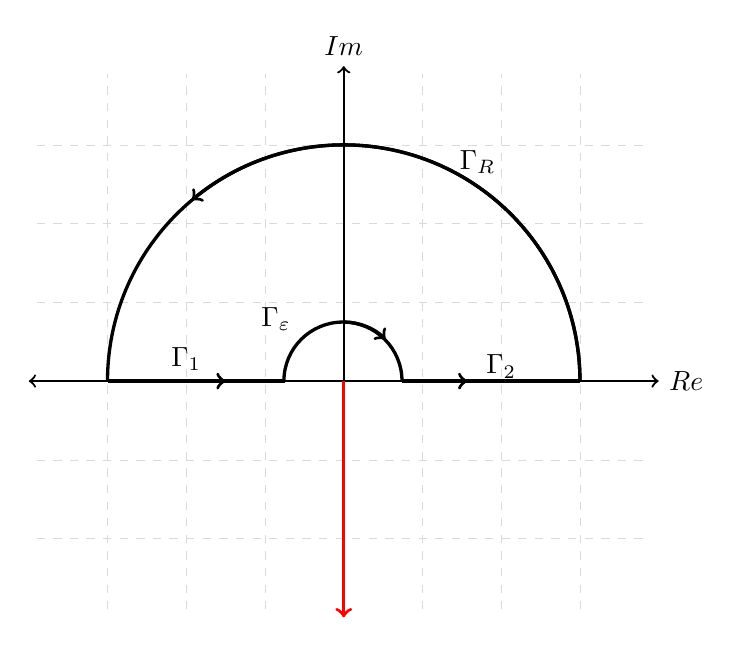
\begin{tikzpicture}
\draw[help lines, color=gray!30, dashed] (-3.9,-2.9) grid (3.9,3.9);
\draw[->,very thick] (3,0) arc (0:130:3cm);
\draw[very thick] (3,0) arc (0:180:3cm) node[above,yshift=2.5cm,xshift=4.7cm]{$\Gamma_R$};
\draw[->,very thick] (0,0.75) arc (90:45:0.75cm);
\draw[very thick] (0.74,0) arc (0:180:0.75cm) node[above,yshift=0.5cm,xshift=-0.1cm]{$\Gamma_\varepsilon$};
\draw[->,very thick] (0.74,0) -- (1.57,0);
\draw[very thick] (0.75,0) -- (3,0) node[above,yshift=-0.1cm,xshift=-1cm]{$\Gamma_2$};
\draw[->,very thick] (-3,0) -- (-1.5,0);
\draw[very thick] (-0.74,0) -- (-3,0) node[above,yshift=0cm,xshift=1cm]{$\Gamma_1$};
\draw[<->, thick] (-4,0)--(4,0) node[right]{$Re$};
\draw[->, thick] (0,0)--(0,4) node[above]{$Im$};
\draw[->,very thick,red] (0,0) -- (0,-3);
\end{tikzpicture}
\end{center}

Let \begin{align*}
    I_1&=\int_{\Gamma_1}\frac{\log^2 z}{z^2+1}dz\\
    I_2&=\int_{\Gamma_2}\frac{\log z}{z^2+1}dz\\
    I_\varepsilon&=\int_{\Gamma_\varepsilon}\frac{\log z}{z^2+1}dz\\
    I_R&=\int_{\Gamma_R}\frac{\log z}{z^2+1}dz
\end{align*}

Note that \begin{align*}
    I_1&=\int_{-R}^{-\varepsilon}\frac{\log^2x}{1+x^2}dx\\
    &=\int_R^\varepsilon\frac{-(\log x+\pi i)^2}{1+x^2}dx\\
    &=\int_\varepsilon^R\frac{\log^2x+2\pi i\log x-\pi^2}{1+x^2}dx\\
    &=I_2+2\pi i\int_\varepsilon^R\frac{\log x}{1+x^2}dx-\pi^2\int_\varepsilon^R\frac{1}{1+x^2}dx\\
    &=I_2-\pi^2(\tan^{-1}(R)-\tan^{-1}(\varepsilon))+2\pi i\int_\varepsilon^R\frac{\log x}{1+x^2}dx
\end{align*}

Now, \begin{align*}
    |I_R|&=\left|\int_{\Gamma_R}\frac{\log^2 z}{1+z^2}dz\right|\\
    &\le\int_0^\pi\frac{R|\log R+i\theta|^2}{R^2-1}d\theta\\
    &\le \pi\frac{R\log^2 R+2R\pi\log R+R\pi^2}{R^2-1}\to0\qquad R\to\infty
\end{align*}
 since $$\lim_{R\to\infty}\frac{\log^2R}{R}=\lim_{R\to\infty}\frac{2\log R}{R}=\lim_{R\to\infty}\frac{2}{R}=0$$ by L'Hopital's Rule and similarly, $\frac{\log R}{R}\to0$.

 Similarly, \begin{align*}
     |I_\varepsilon|&\le \int_\pi^0\frac{\varepsilon|\log\varepsilon+i\theta|^2}{\varepsilon^2-1}d\theta\\
     &\le \pi\frac{\varepsilon\log^2 \varepsilon+2\varepsilon\pi\log \varepsilon+\varepsilon\pi^2}{\varepsilon^2-1}\to0\qquad \varepsilon\to0
 \end{align*} since $$\lim_{\varepsilon\to0}\varepsilon\log^2\varepsilon=\lim_{\varepsilon\to0}\frac{2\log \varepsilon}{\frac{-1}{\varepsilon}}=\lim_{\varepsilon\to0}\frac{2}{\frac{1}{\varepsilon}}=0$$ by L'Hopital's Rule.

 Thus, by the Residue Theorem, \begin{align*}
     2\pi i\res_{z=i}\frac{\log^2 z}{z^2+1}&=2\pi i\frac{\log^2(i)}{i+i}\\
     &=\pi\left(i\frac{\pi}{2}\right)^2\\
     &=-\frac{\pi^3}{4}\\
     &=\lim_{R\to\infty}\lim_{\varepsilon\to0}(I_1+I_2+I_\varepsilon+I_R\\
     &=2\int_0^\infty\frac{\log^2 x}{1+x^2}dx-\frac{\pi^3}{2}\\
     \implies \int_0^\infty\frac{\log^2 x}{1+x^2}dx&=\frac{\pi^3}{8}
 \end{align*}

Note that since the residue is real this forces $\displaystyle \int_0^\infty\frac{\log x}{1+x^2}dx=0$.
\end{solution}
\newpage





\begin{problem} $\,$
Denote $\mathbb{D}=\{z\in\mathbb{C}:|z|<1\}.$ Assume that $f:\mathbb{D}\to\mathbb{D}$ is analytic. Show that if $z_1\not=z_2$ are fixed points of $f$ in $\mathbb{D}$, then $f$ is the identity map.
\end{problem}


\begin{solution}$\,$
Since $\mathbb{D}$ is an open simply connected subset of $\mathbb{C}$ which is not all of $\mathbb{C}$, by the Riemann Mapping Theorem, there exists a $g:\mathbb{D}\to\mathbb{D}$ which is analytic, bijective, has an analytic inverse and is such that $g(z_1)=0$. Say $g(z_2)=w$. Then

Then $g\circ f\circ g^{-1}:\mathbb{D}\to\mathbb{D}$ such that $$g(f(g^{-1}(0)))=g(f(z_1))=g(z_1)=0.$$

Furthermore, $$g(f(g^{-1}(w)))=g(f(z_2))=g(z_2)=w$$ and so $$|(g\circ f\circ g^{-1})(w)|=|w|$$ and so by Schwarz's Lemma, $g\circ f\circ g^{-1}=az$ where $|a|=1$. However, since $$g(f(g^{-1}(w)))=w=aw\implies a=1.$$ Namely, $g\circ f\circ g^{-1}$ is the identity map and so $f$ must be the identity map.
\end{solution}


\end{document}
